% The bounded-stack linchpin: a large but FINITE stack bound D collapses the unbounded
% pushdown behaviour into a finite reachable-configuration set — which keeps the Rocq model
% an ordinary Inductive (no coinduction) and gives TLC a finite model. Palette: bound=violet,
% rocq=indigo, tlc=teal.
\documentclass[border=10pt]{standalone}
\usepackage{tikz}
\usepackage{amsmath}
\usepackage{xcolor}
\usetikzlibrary{arrows.meta, positioning}
\definecolor{bound}{HTML}{7C3AED}
\definecolor{rocq}{HTML}{3730A3}
\definecolor{tlc}{HTML}{0D9488}
\definecolor{ink}{HTML}{1E293B}
\begin{document}
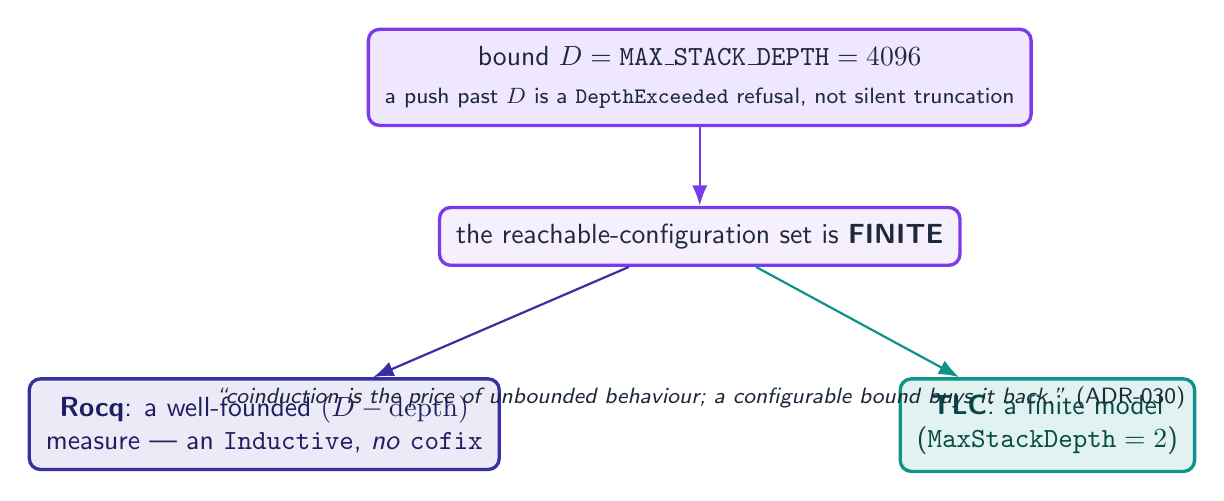
\begin{tikzpicture}[font=\sffamily, >={Latex[length=2.6mm]}, node distance=10mm,
    box/.style={draw, very thick, rounded corners, align=center, inner sep=6pt, text=ink}]

  \node[box, draw=bound, fill=bound!12] (d)
    {bound $D = \texttt{MAX\_STACK\_DEPTH} = 4096$\\[2pt]{\footnotesize a push past $D$ is a \texttt{DepthExceeded} refusal, not silent truncation}};

  \node[box, draw=bound, fill=bound!8, below=of d] (fin)
    {the reachable-configuration set is \textbf{FINITE}};

  \node[box, draw=rocq, fill=rocq!10, below left=14mm and -8mm of fin, text=rocq!60!black] (rocq)
    {\textbf{Rocq}: a well-founded $(D-\mathrm{depth})$\\measure — an \texttt{Inductive}, \emph{no} \texttt{cofix}};
  \node[box, draw=tlc, fill=tlc!12, below right=14mm and -8mm of fin, text=tlc!50!black] (tlc)
    {\textbf{TLC}: a finite model\\($\texttt{MaxStackDepth} = 2$)};

  \draw[->, bound, thick] (d) -- (fin);
  \draw[->, rocq, thick] (fin) -- (rocq);
  \draw[->, tlc, thick]  (fin) -- (tlc);

  \node[ink, font=\sffamily\footnotesize, align=center, below=14mm of fin]
    {\emph{``coinduction is the price of unbounded behaviour; a configurable bound buys it back.''} (ADR-030)};
\end{tikzpicture}
\end{document}
